\chapter{Compensador analógico} \chapterlabel{Informe/6-CompensadorAnalogico} \label{cap:Compensador Analogico}

En este capítulo se analiza la dinámica de la planta que se desea controlar y se utilizan distintas estrategias de análisis y compensación para conseguir que el sistema de levitación presente el comportamiento deseado. 

Como se mencionó en la sección \ref{sec_modelo_estados}, el fenómeno de levitación magnética presenta un comportamiento inestable. Es por ello que se debe implementar un lazo de control que logre estabilizar el sistema. Se propone una estrategia de control mediante la implementación de un lazo de control interno ($G_c$) y luego, mediante un lazo de control externo ($G_{ext}$), mejorar su respuesta temporal. En la figura \ref{fig:diag-en-bloques-comp} se muestra un diagrama en bloques genérico de la compensación planteada.


\begin{figure}[H]
	\centering
	\scalebox{0.8}{\tikzset{%
	buffer/.style={
		draw,
		shape border rotate=270,
		regular polygon,
		regular polygon sides=3,
		fill=blue!20,
		node distance=2cm,
		minimum height=4em
	}
}

\tikzstyle{block} = [draw, fill=blue!20, rectangle, 
minimum height=2.5em, minimum width=3em]

%Acá se define eñ diagrama en bloques completo
\begin{tikzpicture}[auto, node distance=1cm,>=latex']
	% We start by placing the blocks
	\node [input, name=input] {};
	\node [buffer, right=of input](F){F};
	\node [sum, right of=F, node distance=1.5cm] (suma_externa) {+};
	\node [block, right=of suma_externa] (externo) {$G_{ext}$};
	\node [sum, right=of externo] (suma_interna) {+};
	\node[block, right=of suma_interna] (interno) {$G_c$};
	\node [block, right=of interno] (gil) {$G_{IL}$};
	\node [block, right=of gil] (planta) {$G_p$};
	\node [block, below=of interno] (realimentacion_interna) {$H_{estim}$};
	
	\node [block, below=2cm of externo] (realimentacion_externa) {$H_{estim}$};
%	
%	\node [block, right of=suma] (amplificador) {$A(s)$};
	\node [output, right of=planta, node distance=3cm] (output) {};
%	\node [block, below of=amplificador] (realimentacion) {$H(s)$};
%	
%	
%	% Once the nodes are placed, connecting them is easy. 
	\draw [draw,->] (input) -- node[pos=0.2]{$V_{y_{ref}}$} (F);
	\draw [draw,->] (F) -- node[pos=0.9]{$+$}(suma_externa);
	\draw [draw,->] (suma_externa) -- (externo);
	\draw [draw,->] (externo) -- node[pos=0.95]{$+$} (suma_interna);
	\draw [draw,->] (suma_interna) -- (interno);
	\draw [draw,->] (interno) -- (gil);
	\draw [draw,->] (gil) -- (planta);
	\draw [draw,->] (planta) -- node[name=y]{$Y_g$} (output);
%	\draw [draw,->] (amplificador) -- node[name=y]{$V_{deriv}$} (output);
	\draw [->] (y) |- (realimentacion_interna);
	\draw [->] (realimentacion_interna) -| node[pos=0.25]{$V_{estim}$}  node[pos=0.99]{$-$} (suma_interna);
	\draw [->] (y) |- (realimentacion_externa);
	\draw [->] (realimentacion_externa) -| node[pos=0.25]{$V_{estim}$} node[pos=0.99]{$-$} (suma_externa);
\end{tikzpicture}}
	\caption{Diagrama en bloques del compensador propuesto.}	\label{fig:diag-en-bloques-comp}
\end{figure}

\colorbox{red}{poner nombres corrrectos de señales}

\section{Lazo de realimentación interno}

En esta sección se diseña el control del lazo de realimentación interno. Está compuesto por las etapas mostradas en la figura \ref{fig:diag-interno}. Donde $G_c$ corresponde a la transferencia del compensador que se desea diseñar, $G_{IL}$ es la transferencia del controlador de corriente, $G_p$ es la transferencia de la planta y $H_{estim}$ la del estimador de distancia de entrehierro.

\begin{figure}[H]
	\centering
	\tikzset{%
	buffer/.style={
		draw,
		shape border rotate=270,
		regular polygon,
		regular polygon sides=3,
		fill=blue!20,
		node distance=2cm,
		minimum height=4em
	}
}

\tikzstyle{block} = [draw, fill=blue!20, rectangle, 
minimum height=2.5em, minimum width=3em]

%Acá se define eñ diagrama en bloques completo
\begin{tikzpicture}[auto, node distance=1.5cm,>=latex']
	% We start by placing the blocks
	\node [input, name=input] {};
	\node [sum, right of=input, node distance=1.5cm] (suma_interna) {+};
	\node[block, right=of suma_interna] (interno) {$G_c$};
	\node [block, right=of interno] (gil) {$G_{IL}$};
	\node [block, right=of gil] (planta) {$G_p$};
	\node [block, below=of gil] (realimentacion_interna) {$H_{estim}$};
	
	
%	\node [block, right of=suma] (amplificador) {$A(s)$};
	\node [output, right of=planta, node distance=3cm] (output) {};
%	\node [block, below of=amplificador] (realimentacion) {$H(s)$};
%	
%	
%	% Once the nodes are placed, connecting them is easy. 
%	\draw [draw,->] (input) -- node[pos=0.2]{$V_{y_{ref}}$} (F);
	\draw [draw,->] (input) -- node[pos=0.2]{$V_{ref_c}$} node[pos=0.9]{$+$}(suma_interna);

	\draw [draw,->] (suma_interna) -- node{$Ve_{int}$} (interno);
	\draw [draw,->] (interno) -- node{$V_{IL{ref}}$} (gil);
	\draw [draw,->] (gil) -- node{$I_L$} (planta);
	\draw [draw,->] (planta) -- node[name=y]{$Y_g$} (output);
%	\draw [draw,->] (amplificador) -- node[name=y]{$V_{deriv}$} (output);
	\draw [->] (y) |- (realimentacion_interna);
	\draw [->] (realimentacion_interna) -| node[pos=0.25]{$V_{estim}$}  node[pos=0.99]{$-$} (suma_interna);
%	\draw [->] (y) |- (realimentacion_externa);
%	\draw [->] (realimentacion_externa) -| node[pos=0.25]{$V_{estim}$} node[pos=0.99]{-} (suma_externa);
\end{tikzpicture}
	\caption{Diagrama en bloques del lazo de compensación interno.}	\label{fig:diag-interno}
\end{figure}

Las funciones transferencia de cada bloque del diagrama \ref{fig:diag-interno} están dadas por:

\begin{equation*}
	G_{IL}(s) =\frac{I_L[A]}{V_{IL_{ref}}[V]}=\frac{6}{1+\frac{s}{12.17}}
\end{equation*}

\begin{equation*} 
	G_{p}(M,s)=\frac{Y_g[m]}{I_L[A]}=-\sqrt{\frac{30}{M}}*\frac{1.201}{s^{2}-4900}
\end{equation*}

\begin{equation*} 
	H_{estim}(s)=\frac{V_{estim}[V]}{Y_{g}[m]}=\frac{259.6}{(1+\frac{s}{1\:kr/s})}
\end{equation*}

A continuación se analiza la estabilidad de la planta considerando una masa $M=30\:kg$ y se diseña el bloque del compensador interno $G_C(s)$ para lograr estabilizarla. Luego, se verificará la estabilidad con este mismo compensador para una masa $M=1\:kg$, que corresponde a la mínima con la que trabaja el sistema.

\subsection{Análisis de estabilidad}

Para realizar el análisis de estabilidad se parte de las transferencias de la planta $G_{p}(s)$ para una masa de $30\:kg$, del controlador de corriente $G_{IL}(s)$ y del lazo de realimentación $H_{estim}(s)$. A partir de ellas se obtiene la transferencia a lazo abierto total $GH_T(s)$ de la expresión \ref{eq_GT2}.

\begin{equation*}
	GH_T(s)=G_{p}(s)*G_{iL}(s)*H_{estim}(s) 
\end{equation*}

\begin{equation} \label{eq_GT2}
		GH_T(s)=\frac{0.38}{(1-(\frac{s}{70\:r/s})^2)(1+\frac{s}{12.17\:r/s })(1+\frac{s}{1\:kr/s}) }	
\end{equation}



Para comenzar el análisis se considera un compensador $G_c=K$, donde K es una constante positiva. Por lo tanto, se plantea la transferencia de lazo abierto:

\begin{equation} \label{eq_GT3}
	G_c*GH_T(s)=\frac{K*0.38}{(1-(\frac{s}{70\:r/s})^2)(1+\frac{s}{12.17\:r/s })(1+\frac{s}{1\:kr/s}) }	
\end{equation}

Utilizando la transferencia de la ecuación \ref{eq_GT3}, con $K=1$, se  grafican los diagramas de Bode y de Nyquist y, a partir de ellos, se analizará la estabilidad. Estos se muestran en las figuras \ref{fig:Diag_Bode_lazo_abierto_30kg} y \ref{fig:Diag_Nyquist_lazo_abierto_30kg} respectivamente.

\begin{figure}[H]
	\centering
	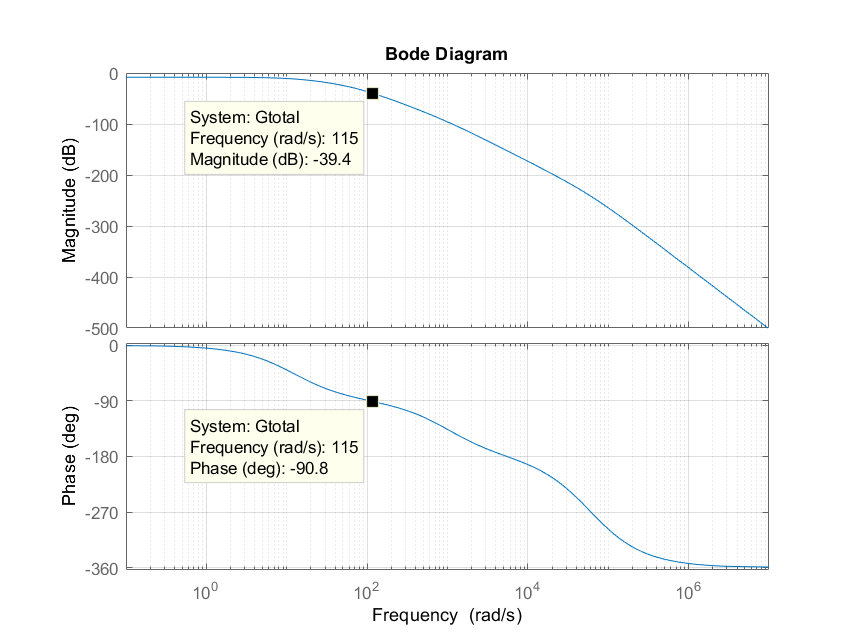
\includegraphics[scale=0.8]{bode_planta_30kg.png}
	\caption{Diagrama de Bode de lazo abierto $G_c*GH_T$ con $M=\:30 kg$.}
	\label{fig:Diag_Bode_lazo_abierto_30kg}
\end{figure}

\begin{figure}[H]
	\centering
	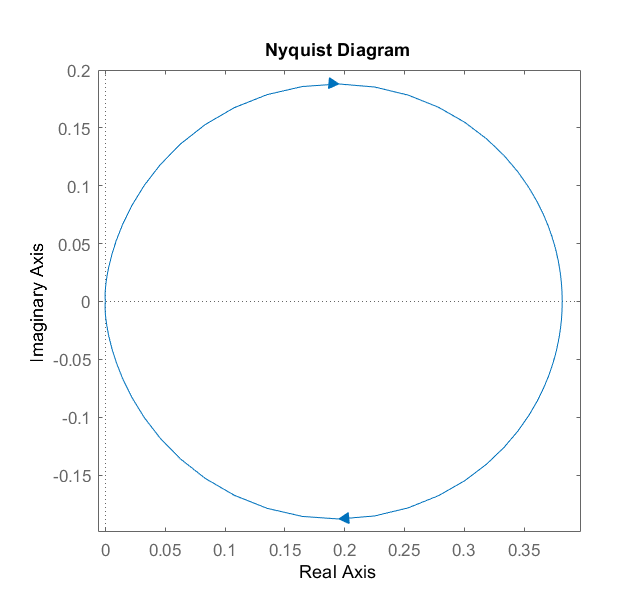
\includegraphics[scale=0.6]{nyquist_planta_30kg.png}
	\caption{Diagrama de Nyquist de $G_c*GH_T$ con $M=30\:kg$.}
	\label{fig:Diag_Nyquist_lazo_abierto_30kg}
\end{figure}


%\noindent Con la transferencia de la ecuación  \ref{eq_GT2} se  grafica el diagrama de Bode  en la figura \ref{fig:Diag_Bode_lazo_abierto_30kg}. El criterio de estabilidad de Bode dice que para determinar la estabilidad de un sistema en un diagrama de Bode se debe observar si la magnitud es mayor a 0dB antes de que la fase alcance -180º. En este caso nuestro sistema es de no mínima fase... \colorbox{red}{ver si dejamos esto o vamos directo a nyquist}

Como la transferencia de la planta $GH_T$ tiene un polo en el semiplano derecho del plano "S" no es posible determinar su estabilidad por medio del diagrama de Bode. Por lo tanto, se analiza la estabilidad por medio del criterio de Nyquist.

Como se observa en el diagrama en bloques de la figura \ref{fig:diag-interno}, para compensar al sistema se planteó una realimentación negativa. Por lo tanto, para analizar su estabilidad según Nyquist se deben determinar la cantidad de giros (N) de $G_c*GH_T$ alrededor del punto $-1+j0$ en la figura \ref{fig:Diag_Nyquist_lazo_abierto_30kg} y la cantidad de polos (P) en el semiplano derecho de la función transferencia $G_c*GH_T$. El sistema resultará estable si se cumple la condición \ref{eq_condicion_Nyquist}, donde Z representa la cantidad de ceros en el semiplano derecho de $1+G_c*GH_T(s)$.

\begin{equation}\label{eq_condicion_Nyquist}
	Z=N+P=0
\end{equation}


Debido a que $GH_T$ tiene un polo en el semiplano derecho ($P=1$) y no hay giros alrededor del punto $-1+j0$ ($N=0$), resulta que $Z=1$. Por lo tanto, la transferencia de lazo cerrado ($TLC_{interna}$) presenta un comportamiento inestable. En la figura \ref{fig:Diag_Nyquist_lazo_abierto_30kg} se puede observar que no existe ningún valor de $K>0$ que haga que el contorno de $G_c*GH_T$ rodee el punto $-1+j0$. Por lo tanto, se propone implementar un compensador con $K<0$, para invertir el contorno de $G_c*GH_T$. Esto resulta equivalente a considerar $K>0$ y usar realimentación positiva en el lazo de control interno. De esta forma se obtiene el diagrama en bloques de la figura \ref{fig:diag-interno_realimentacion_positiva}.


\begin{figure}[H]
	\centering
	\tikzset{%
	buffer/.style={
		draw,
		shape border rotate=270,
		regular polygon,
		regular polygon sides=3,
		fill=blue!20,
		node distance=2cm,
		minimum height=4em
	}
}

\tikzstyle{block} = [draw, fill=blue!20, rectangle, 
minimum height=2.5em, minimum width=3em]

%Acá se define eñ diagrama en bloques completo
\begin{tikzpicture}[auto, node distance=1.5cm,>=latex']
	% We start by placing the blocks
	\node [input, name=input] {};
	\node [sum, right of=input, node distance=1.5cm] (suma_interna) {+};
	\node[block, right=of suma_interna] (interno) {$G_c$};
	\node [block, right=of interno] (gil) {$G_{IL}$};
	\node [block, right=of gil] (planta) {$G_p$};
	\node [block, below=of gil] (realimentacion_interna) {$H_{estim}$};
	
	
%	\node [block, right of=suma] (amplificador) {$A(s)$};
	\node [output, right of=planta, node distance=3cm] (output) {};
%	\node [block, below of=amplificador] (realimentacion) {$H(s)$};
%	
%	
%	% Once the nodes are placed, connecting them is easy. 
%	\draw [draw,->] (input) -- node[pos=0.2]{$V_{y_{ref}}$} (F);
	\draw [draw,->] (input) -- node[pos=0.2]{$Vref2$} node[pos=0.9]{+}(suma_interna);

	\draw [draw,->] (suma_interna) -- node{$Ve2??$} (interno);
	\draw [draw,->] (interno) -- node{$V_{IL{ref}}$} (gil);
	\draw [draw,->] (gil) -- node{$I_L$} (planta);
	\draw [draw,->] (planta) -- node[name=y]{$Y_g$} (output);
%	\draw [draw,->] (amplificador) -- node[name=y]{$V_{deriv}$} (output);
	\draw [->] (y) |- (realimentacion_interna);
	\draw [->] (realimentacion_interna) -| node[pos=0.25]{$V_{estim}$}  node[pos=0.99]{-} (suma_interna);
%	\draw [->] (y) |- (realimentacion_externa);
%	\draw [->] (realimentacion_externa) -| node[pos=0.25]{$V_{estim}$} node[pos=0.99]{-} (suma_externa);
\end{tikzpicture}
	\caption{Diagrama en bloques del lazo de compensación interno considerando realimentación positiva.}	\label{fig:diag-interno_realimentacion_positiva}
\end{figure}

Siguiendo el criterio de estabilidad de Nyquist, al utilizar realimentación positiva, la cantidad de giros (N) debe analizarse alrededor del punto $1+j0$. Si estos son en sentido horario, N será positivo, caso contrario será negativo. Al variar el valor de K, es posible hacer que el punto $1+j0$ quede contenido en la zona 1 o en la zona 2 de la figura \ref{fig:nyquist-con-zonas}. 

\begin{figure}[H]
	\centering
	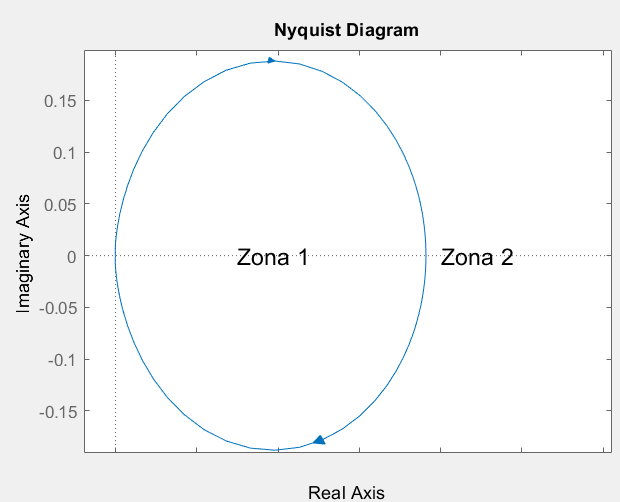
\includegraphics[scale=1]{nyquist_con_zonas.png}
	\caption{Diagrama de Nyquist con zonas marcadas.}	
	\label{fig:nyquist-con-zonas}
\end{figure}

Si el punto queda dentro de la zona 1, el número de giros es $N=1$. Por lo tanto, se plantea:

\begin{equation*}
	Z = N + P = 2
\end{equation*}


Si el punto queda dentro de la zona 2, el número de giros es $N=0$. Por lo tanto, se plantea:

\begin{equation*}
	Z = N + P = 1
\end{equation*}

Debido a que en ambas zonas Z resulta mayor que cero, el sistema realimentado no puede ser estabilizado con ningún valor K. Para lograrlo se debe generar una zona en el diagrama de Nyquist donde exista un giro alrededor de $1 + j0$ en sentido antihorario. Para ello, es necesario aumentar la fase para que pueda superar el valor de 0$\mathrm{{}^\circ}$.  Para que esto se cumpla, el diagrama de Nyquist debe tener una forma como la  mostrada en la figura \ref{fig:nyquist-deseado-analog}.

\colorbox{red}{Agregar las zonas en la imagen}

\begin{figure}[H]
	\centering
	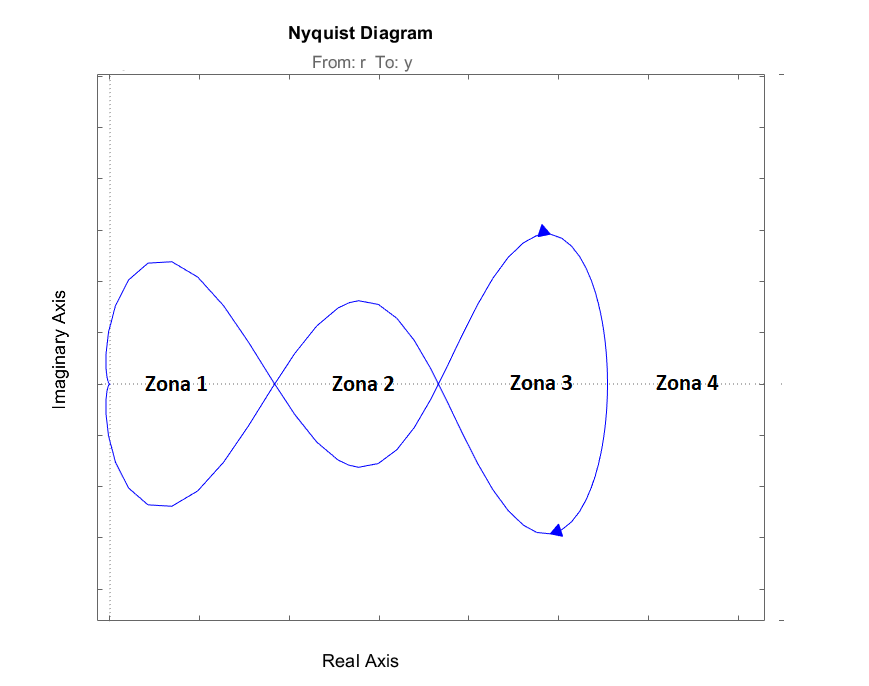
\includegraphics[scale=0.6]{Nyquist-deseado-analog.png}
	\caption{Forma del diagrama de Nyquist deseado.}
	\label{fig:nyquist-deseado-analog}
\end{figure}

De esta manera se generan cuatro zonas. Sin embargo, solo en la zona 2 se genera un giro en sentido antihorario ($N=-1$) como es deseado, por lo que resulta:

\begin{equation*}
	Z = N + P = 0
\end{equation*}

%Para lograr el comportamiento del sistema como en la figura 	\ref{fig:nyquist-deseado-analog} se debe tener en cuenta que el m\'{o}dulo de la transferencia de lazo abierto en el primer cruce de la fase por 0$\mathrm{{}^\circ}$ debe ser mayor a $0\:dB$ y, en el segundo cruce, menor. Para ello, se propone implementar un compensador por adelanto de fase.

Por lo tanto, para lograr que el diagrama de Nyquist tenga la forma deseada, se propone implementar un compensador por adelanto de fase.

\colorbox{red}{Ver como terminaomos esta seccion y la enganchamos con la que viene}


\subsection{Diseño de la red de adelanto de fase}

Para lograr el comportamiento del sistema como en la figura 	\ref{fig:nyquist-deseado-analog} se debe tener en cuenta que el m\'{o}dulo de la transferencia de lazo abierto en el primer cruce de la fase por 0$\mathrm{{}^\circ}$ debe ser mayor a $0\:dB$ y, en el segundo cruce, menor. 

De esta forma, al observar la figura \ref{fig:Diag_Bode_lazo_abierto_30kg} se decide adelantar la fase 100º en aproximadamente $200\:r/s$. Esto se logra mediante el uso de dos redes de adelanto de fase de 65$\mathrm{{}^\circ}$ cada una. 


\noindent De esta forma, las ecuaciones de dise\~{n}o resultan:

\begin{equation*}
	\begin{aligned}
		&W_0 =200\:r/s\\
		&{\varphi }_{max} =65\textrm{º}\\
		&\alpha =\frac{1+sen({\varphi }_{max})}{1-sen{(\varphi }_{max})}=20.346491\\
		&W_c =\frac{W_0}{\sqrt{\alpha }}=\ 44.3\:r/s\\
		&W_p =\sqrt{\alpha }*W_0=902.1\: r/s\\
	\end{aligned}
\end{equation*} 
\noindent Finalmente, se llega a la transferencia del controlador:

\colorbox{red}{Ponemos la transferencia generica del controlador? Pq nunca hicimos referencia a donde van alpha, W0, Wc...}

\begin{equation}  
	G_c(s)=K*{[20.346*\frac{(s+44.3)}{(s+902.1)}]}^2
\end{equation} 

\noindent En la figura \ref{fig:bode-analog-compensado-para-k-1} se muestra el diagrama de bode de ${GH}_T*G_C$ con $K=1$. Se puede observar que la ganancia $K$ puede adoptar valores desde $15.7\:dB$ hasta $35.5\:dB$ aproximadamente. Al considerar que el sistema debe soportar una masa variable entre $1\:kg$ y $30\:kg$, y que la ganancia de la transferencia de la planta para $1\:kg$ es de $5.5$ veces ($14\:dB$) mayor que para $30\:kg$, se debe adoptar una ganancia del compensador que mantenga la estabilidad para estos dos casos. Es decir, la ganancia m\'{i}nima es de $15.7\:dB$ y la m\'{a}xima es de $35.5\:dB - 14\:dB = 21.5\:dB$. Por lo tanto, se elige que el cruce por cero de la ganancia se encuentre ahora en $88\:r/s$, lo que significa que $K=20\:dB\ \equiv \ 10\: veces$.


\begin{figure}[H]
	\centering
	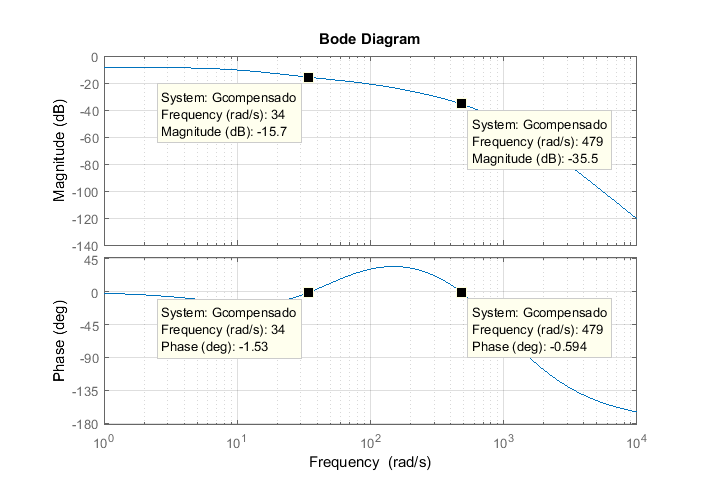
\includegraphics[scale=0.85]{Bode-k-1-M-30.png}
	\caption{Diagrama de Bode de $GH_T*G_C$ para $K=1$ y $M=30\:kg$.}
	\label{fig:bode-analog-compensado-para-k-1}
\end{figure}

\noindent En la figura \ref{fig:bode-analog-compensado-para-k-10} se muestra el diagrama de Bode al considerar la ganancia del compensador. En ella se puede observar que se  cumple con el criterio de estabilidad, puesto que en el primer cruce por 0º, la magnitud es mayor a 0 dB y en el segundo cruce, menor. Adem\'{a}s, en la figura \ref{fig:nyquist-analog-para-k-10} se puede ver que la forma del diagrama de Nyquist es como la deseada.

\begin{figure}[H]
	\centering
	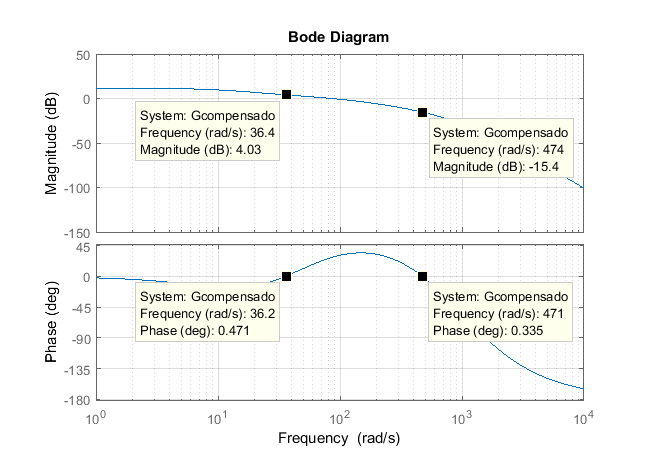
\includegraphics[scale=0.8]{Bode-k-10-M-30.png}
	\caption{Diagrama de Bode de $GH_{T}*G_C$ para $K=10$ y $M=30\:kg$.}
	\label{fig:bode-analog-compensado-para-k-10}
\end{figure}

\begin{figure}[H]
	\centering
	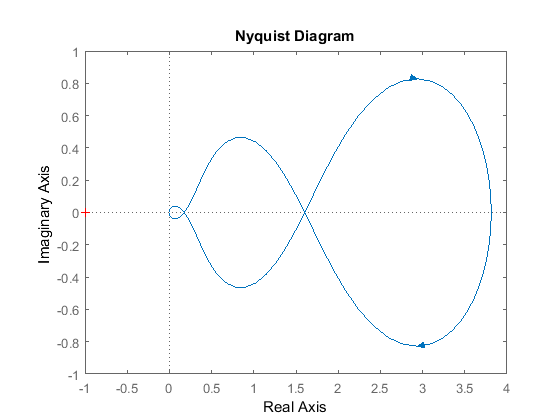
\includegraphics[scale=0.8]{Nyquist-k-10-M-30.png}
	\caption{Diagrama de Nyquist de $GH_T*G_C$ para $K=\:10$ y $M=30\:kg$.}
	\label{fig:nyquist-analog-para-k-10}
\end{figure}

\subsection{Transferencia de lazo cerrado}

Finalmente se puede expresar la función transferencia del lazo de control interno como:
%
%-3.6301e05 (s+1000) (s+44.3)^2
%------------------------------------------------------------------
%(s+304.3) (s+115.6) (s^2 + 44.84s + 2588) (s^2 + 2352s + 1.498e06)

\colorbox{red}{escribir tlc, o mostrar ganancia en contínua que es negativ}

\begin{equation}
	TLC_{interna}(s)=\frac{Y_g}{V_{ref_c}}=\frac{G_c*G_{p}*G_{iL}}{1-G_c*G_{p}*G_{iL}*H_{estim}}
	%	\frac{-3.6301*}{den}
\end{equation}

\begin{equation}
	TLC_{interna}(s)=\frac{-3.6301*10^5(s+1000)(s+44.3)^2}{(s+304.3) (s+115.6) (s^2 + 44.84s + 2588) (s^2 + 2352s + 1.498*10^6)}	
\end{equation}

\colorbox{red}{Conviene hacer el lugar de raices de la TLC?}
%Por último se simuló la respuesta del sistema a un escalón de amplitud unitaria en la señal $V_{ref_c}$. La salida es un valor de distancia de entrehierro $Y_g$ en metros. En la figura \ref{fig:rta-escalon-k-10-m-30} se puede observar la respuesta al escalón del sistema con masa de $30\:kg$.
%
%\colorbox{red}{Ver como acomodar lo de la respuesta al escalon (y para 1kg tambien)}
%
%\begin{figure}[H]
%	\centering
%	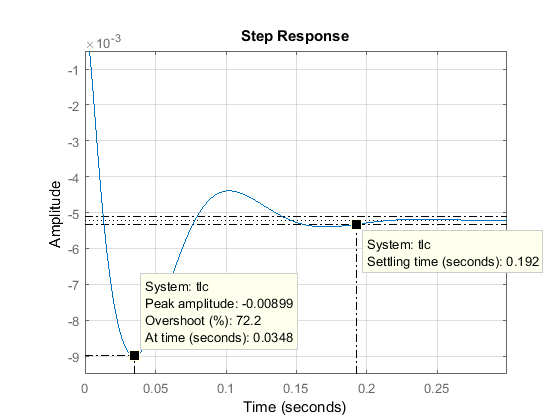
\includegraphics[scale=0.80]{Respuesta-al-escalon-K-10-M-30Kg.png}
%	\caption{Respuesta al escalón para $M=30\:kg$.}
%	\label{fig:rta-escalon-k-10-m-30}
%\end{figure}

\subsection{Verificación de estabilidad con masa de 1 kg}

%\noindent Se verifica la estabilidad del sistema  para el caso en que la masa sea de $1\:kg$ con el compensador dise\~{n}ado para el caso de masa m\'{a}xima. Para ello, se analizan los diagramas de Bode y Nyquist mostrados en las figuras \ref{fig:bode-analog-para-M-1Kg} y \ref{fig:nyquist-analog-para-M-1Kg}. Adem\'{a}s, en la figura \ref{fig:respuesta-analog-al-escalon-para-M-1Kg} puede observarse la respuesta al escal\'{o}n. A partir de ellos, es posible verificar que el sistema resulta estable para todo el rango de masas en el que opera el sistema. 

\noindent Se verifica la estabilidad del sistema  para el caso en que la masa sea de $1\:kg$ con el compensador dise\~{n}ado para el caso de masa m\'{a}xima. Para ello, se analizan los diagramas de Bode y Nyquist mostrados en las figuras \ref{fig:bode-analog-para-M-1Kg} y \ref{fig:nyquist-analog-para-M-1Kg}. A partir de ellos, es posible verificar que el sistema resulta estable para todo el rango de masas en el que opera el sistema. Sin embargo, se puede observar que el margen de fase es menor que 45º, por lo que el sistema puede presentar un transitorio con oscilaciones amortiguadas. A raiz de esto, se propone implementar un lazo de control externo que permita mejorar dicha respuesta.

\begin{figure}[H]
	\centering
	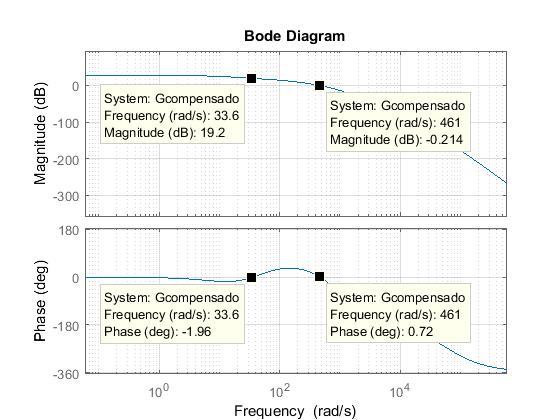
\includegraphics[scale=0.80]{bodecompensado1kg.png}
	\caption{Diagrama de Bode de $GH_T*G_c$ para $M=1\:kg$.}
	\label{fig:bode-analog-para-M-1Kg}
\end{figure}
\colorbox{red}{Ver sis e puede quitar el fondo de la imagen..}

\begin{figure}[H]
	\centering
	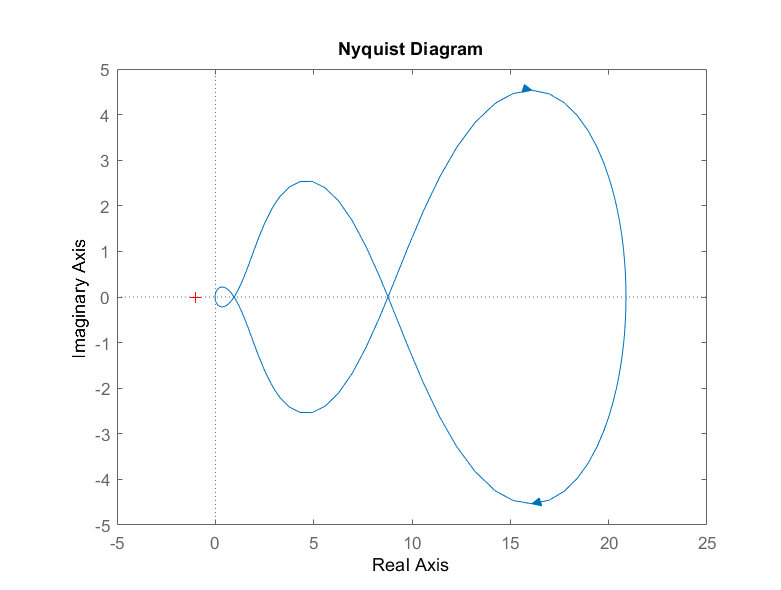
\includegraphics[scale=0.55]{nyquistcompensado1kg.png}
	\caption{Diagrama de Nyquist de $GH_T*G_C$ para $M=1\:kg$.}
	\label{fig:nyquist-analog-para-M-1Kg}
\end{figure}

%\begin{figure}[H]
%	\centering
%	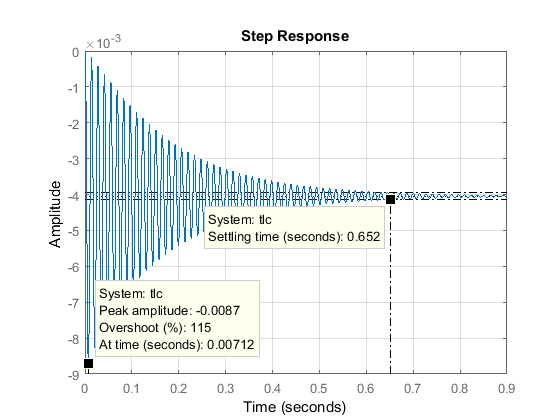
\includegraphics[scale=0.80]{rtaescaloncompensado1kg.png}
%	\caption{Respuesta al escalón para $M=1\:kg$.}
%	\label{fig:respuesta-analog-al-escalon-para-M-1Kg}
%\end{figure}



\section{Lazo de realimentación externo}

\noindent Se plantea un lazo de realimentación externo como se muestra en la  figura \colorbox{red}{poner referencia a imagen del diagrama simplificada}. En el lazo de realimentación interno actúa el compensador por adelanto de fase diseñado previamente y, en el externo, un controlador del tipo integral. Esto permite suavizar la respuesta al escalón del sistema y eliminar el error en régimen permanente.


\noindent Para el an\'{a}lisis se considera como realimentaci\'{o}n: 

\[H_{estim}=\frac{V_{estim}}{Y_g[m]}= \frac{259.6}{(1 + \frac{s}{1\:k})
}\] 

\noindent La cadena de avance con masa de $30\:kg$ es:

\begin{equation} \label{eq_cadena_avance_integrador}
	G[M=30]=TLC_{interna}(s)[M=30]*G_{integ}
\end{equation}


Inicialmente se plantea un compensador del tipo integrador cuya transferencia es de la forma:
\begin{equation}
	G_{integ}= \frac{k_{int}}{s}
\end{equation}

El problema de este integrador es que presenta una ganancia infinita en continua. Por lo tanto, se propone implementar un compensador con un polo ($p_{int}$) en baja frecuencia, que actúe como integrador a las frecuencias de la planta, pero que tenga ganancia finita en continua. De esta forma, se decide ubicar el polo en $0.1\:rad/s$ y la transferencia a implementar resulta:

\begin{equation}
	G_{integ}=\frac{k_{int}}{1+\frac{s}{p_{int}}}=\frac{k_{int}}{1+\frac{s}{0.1\:r/s}}	
\end{equation}

Sin embargo, es importante tener en cuenta que la ubicación de un polo en baja frecuencia provoca que la cancelación del error en régimen permanente no sea completa.

\colorbox{red}{Ver de verificar el error al escalón mas adelante y referenciarlo a esta parte}
%, pero de todas maneras sea pequeña en comparación con la distancia de separación.

%Debido a que no usamos un integrador ideal, la respuesta al escalón presentará un cierto error.
Para encontrar el valor adecuado de $k_{int}$ se grafica el lugar de raíces de la expresión \ref{eq_cadena_avance_integrador} considerando $k_{int}=1$. Este puede verse en la figura \ref{fig:lugar-de-raices-con-integrador-analog}.



\colorbox{red}{hacer imagen de lugar de raices con realimentacin negativa}

\begin{figure}[H]
	\centering
	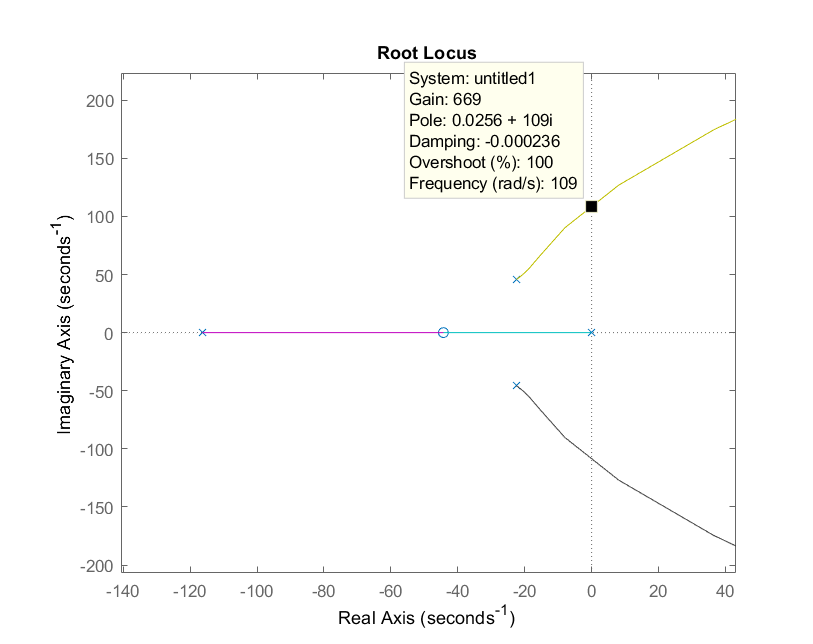
\includegraphics[scale=0.5]{rlocusconintegrador30kg.png}
	\caption{Lugar de raíces con el integrador.}
	\label{fig:lugar-de-raices-con-integrador-analog}
\end{figure}

A partir del lugar de raíces se puede determina que el sistema resulta inestable para cualquier valor de $k_{int}>0$ puesto que la TLC interna del sistema presenta una ganancia negativa. Por lo tanto, debe utilizarse un valor de $k_{int}>0$, o bien seguir con $k_{int}>0$ pero con realimentación positiva. 

Por lo tanto, al considerar una ganancia para el integrador $k_{int}>0$ y realimentación positiva se plantea el diagrama en bloques de la figura \colorbox{red}{asdasd}.

\colorbox{red}{Agregar diagrama en bloqeus con realimentación positiva del lazo externo}

EL lugar de raíces resulta:

\begin{figure}[H]
	\centering
	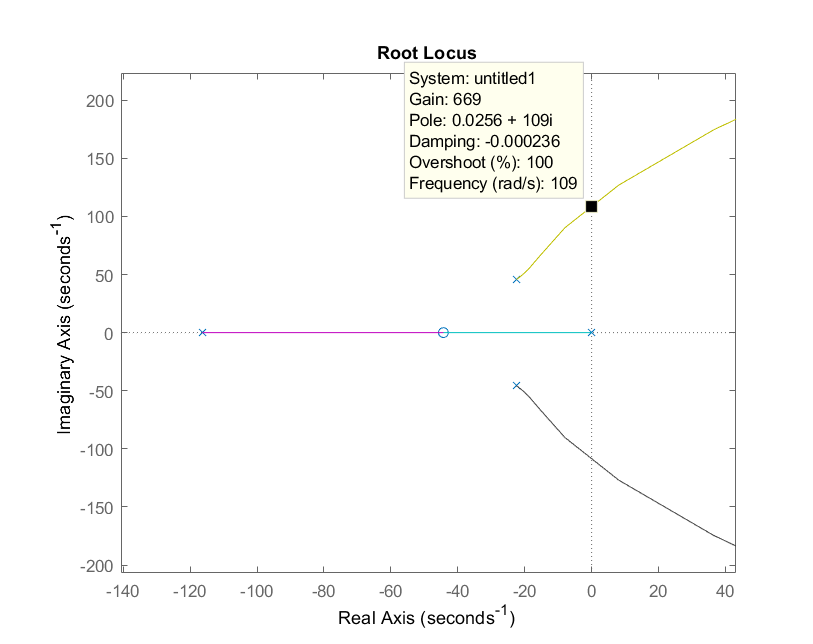
\includegraphics[scale=0.5]{rlocusconintegrador30kg.png}
	\caption{Lugar de raíces con el integrador.}
	\label{fig:lugar-de-raices-con-integrador-analog}
\end{figure}
 
\noindent En la figura \ref{fig:lugar-de-raices-con-integrador-analog} se puede observar que, para que se mantenga la estabilidad del sistema, la ganancia del integrador ($k_{int}$) debe ser menor a 669. Teniendo esto en cuenta, en la figura \ref{fig:respuesta-al-escalon-con-k-1-M-30-analog} se muestra la respuesta al escalón del sistema compensado con el integrador para una ganancia de $k_{int}=1$. Es posible observar que, si bien no presenta oscilaciones, el tiempo de establecimiento es de aproximadamente $16.6 \:s$. Por lo tanto, se decide aumentar el valor de ganancia hasta obtener una relación aceptable entre el tiempo de respuesta y el sobrepico.

\begin{figure}[H]
	\centering
	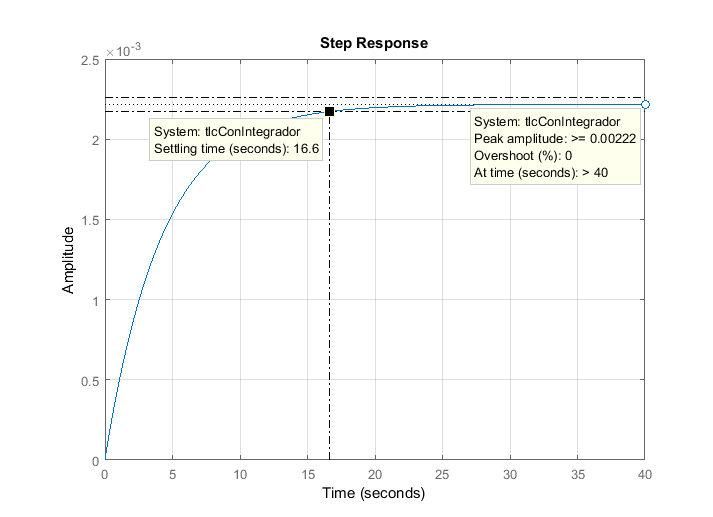
\includegraphics[scale=0.85]{stepresponseintegradorkint_1_m_30.png}
	\caption{Respuesta al escalón con integrador con $K_{int} =1$ y $M=30\:kg$.}
	\label{fig:respuesta-al-escalon-con-k-1-M-30-analog}
\end{figure}

\noindent En la figura \ref{fig:respuesta-al-escalon-con-k-50-M-30}, se observa la respuesta al escalón para una ganancia del integrador de $k_{int}=50$ que resulta en un tiempo de establecimiento de $0.6\:s$ y un sobrepico de 0\%. Por lo tanto, se adopta este valor de ganancia para el diseño del integrador.

\begin{figure}[H]
	\centering
	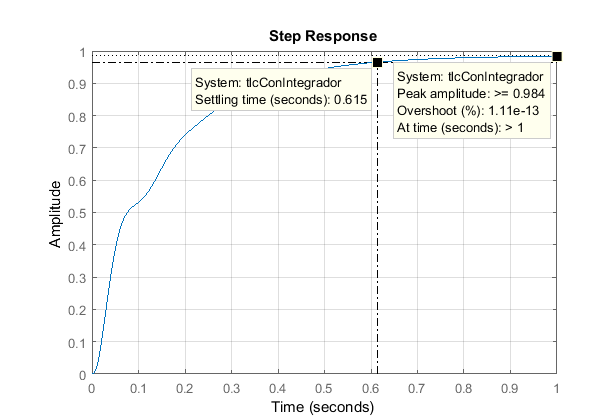
\includegraphics[scale=0.85]{stepresponseintegradorkint_50_m_30.png}
	\caption{Respuesta al escalón con integrador para $K_{int}=50$ y $M = 30\:kg$.}
	\label{fig:respuesta-al-escalon-con-k-50-M-30}
\end{figure}

\noindent La respuesta al escal\'{o}n cuando la masa es de $1 \:kg$ se muestra en la figura \ref{fig:respuesta-al-escalon-con-k-50-M-1}. All\'{i} se puede observar que el tiempo de establecimiento es de $0.74\:s$ y que no presenta sobrepicos.

\begin{figure}[H]
	\centering
	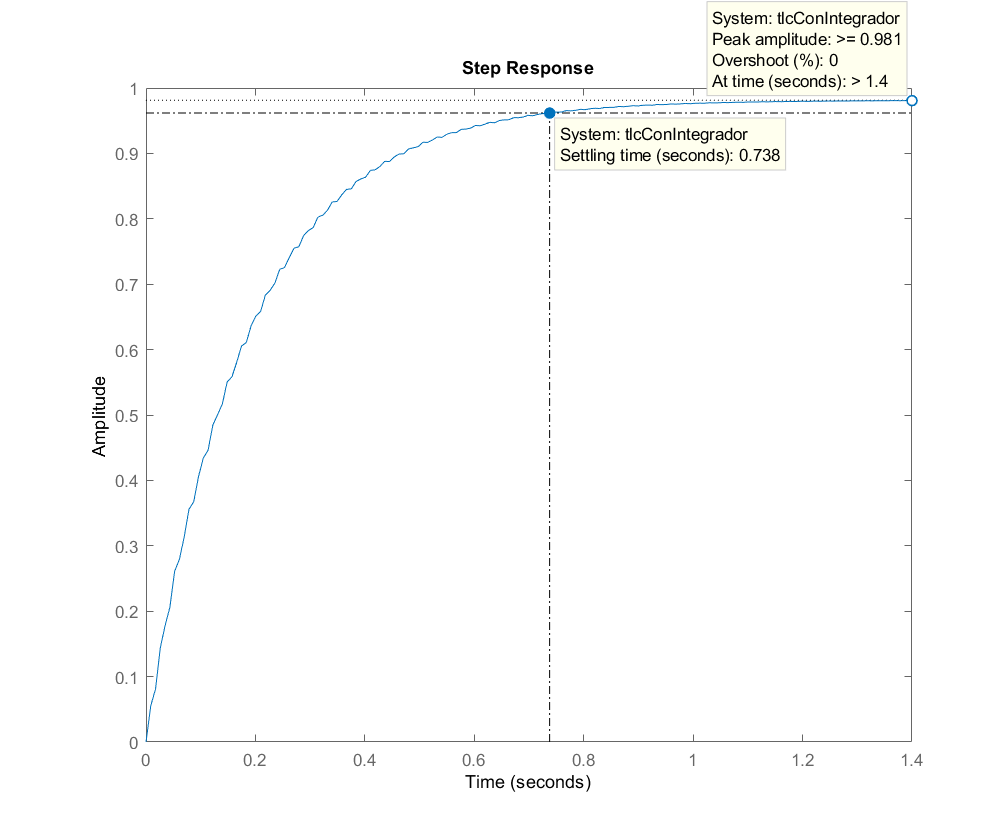
\includegraphics[scale=0.85]{stepresponseintegradorkint_50_m_1.png}
	\caption{Respuesta al escalón con integrador para $K_{int} =50$ y $M = 1 \:kg$.}
	\label{fig:respuesta-al-escalon-con-k-50-M-1}
\end{figure}

\colorbox{red}{Poner TLC externa}

\section{Implementación circuital}

\subsection{Implementación circuital de la red de adelanto de fase}

\noindent Para cada etapa del compensador por adelanto se utiliza la topología mostrada en la figura \ref{fig:red-adelanto-fase}. Consiste en  un polo y un cero con ganancia unitaria (si Ra = Rb). Luego, se agrega la ganancia como una etapa separada.

\begin{figure}[H]
	\centering
	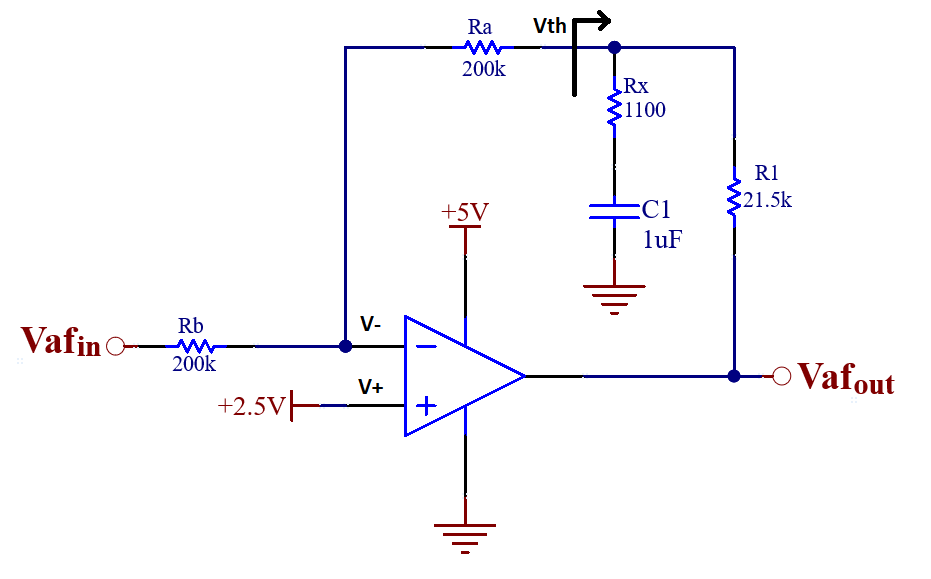
\includegraphics[scale=0.55]{Red-adelanto-fase.png}
	\caption{Diseño circuital de una red de adelanto de fase.}
	\label{fig:red-adelanto-fase}
\end{figure}

\noindent La transferencia de lazo cerrado de esta etapa es:

\begin{equation} 
	\frac{V_{out}}{V_{in}}= - \frac{R_a}{R_b}*\frac{1+sC(R_x+R_1)}{1+sCR_x}
\end{equation}

\noindent Por lo tanto, para tener un polo en $902.1\:Hz$ y un cero en $44.3\:Hz$, al elegir un capacitor $C = 1\:uF$, resulta en $R_x = 1100\:\Omega$ y $R_1 = 21.5\:k\Omega$. Además, se elige $R_a = R_b = 200\:k\Omega$ para obtener una ganancia unitaria. Luego, la ganancia del compensador se obtiene con una etapa amplificadora.
Para ello, se utiliza el circuito mostrado en la figura \ref{fig:ganancia-compensador}. Para lograr una ganancia de $K=10$ se utiliza $R_{322} = 1\:k\Omega$ y $R_{323} = 10\:k\Omega$.


\begin{figure}[H]
	\centering
	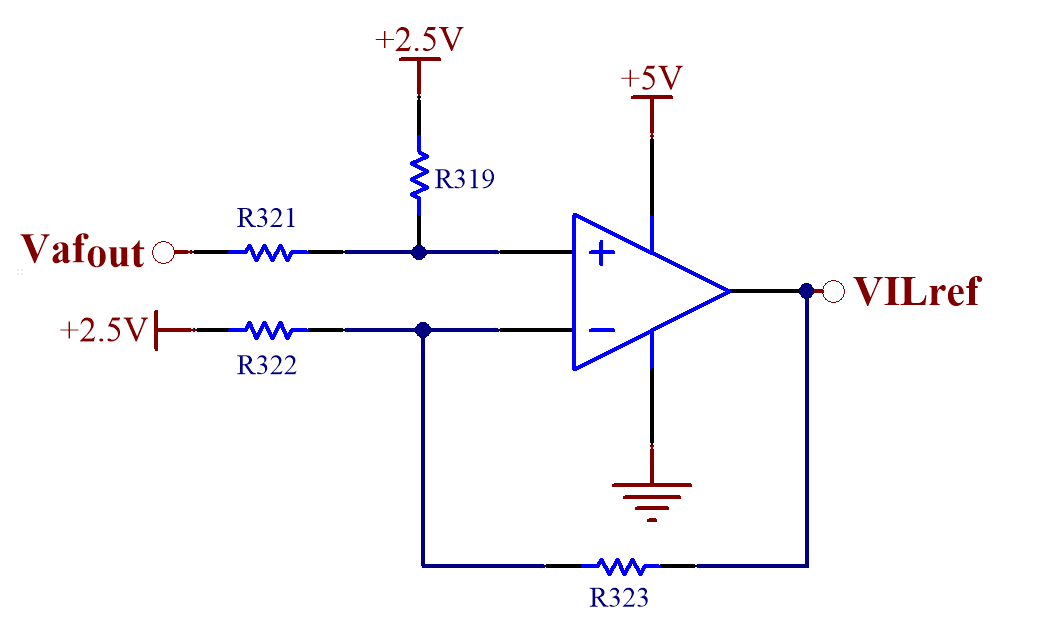
\includegraphics[scale=0.6]{Ganancia-compensador.png}
	\caption{Etapa de ganancia del compensador.}
	\label{fig:ganancia-compensador}
\end{figure}

\subsection{Implementación circuital del integrador}

\noindent En la figura \ref{fig:circuito-integrador} se puede observar la topología y los valores utilizados en cada componente para el diseño del circuito integrador. 

\begin{figure}[H]
	\centering
	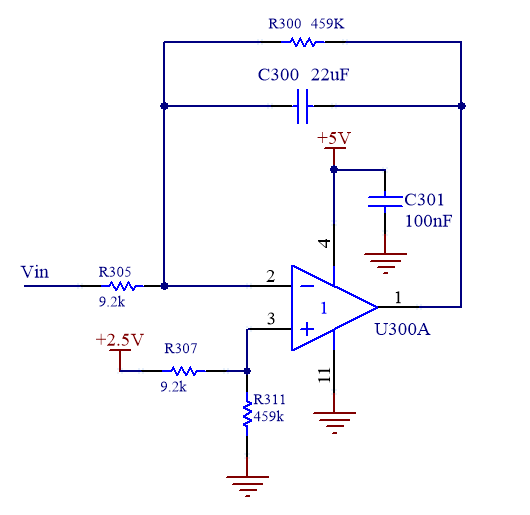
\includegraphics[scale=0.6]{Circuito-integrador.png}
	\caption{Implementación circuital del integrador.}
	\label{fig:circuito-integrador}
	\end{figure}
\section{Etapa de entrada}
\subsection{Cálculo de ganancia de entrada}

\noindent La ganancia de la TLC correspondiente a la ganancia de contínua total de los bloques con el integrador ya incorporado, resulta:

\begin{equation} 
	G_{TLC_{final}} \simeq \frac{1}{H_{estim}} = - \frac{1}{259.6}
\end{equation}

\begin{figure}[H]
	\centering
	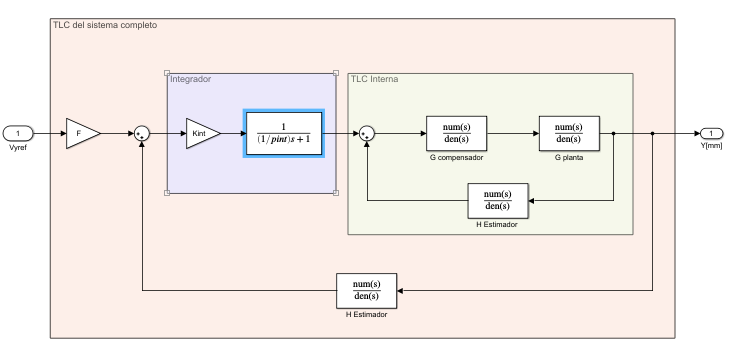
\includegraphics[scale=0.8]{Diagrama-en-bloques-compensador.png}
	\caption{Diagrama en bloques final.}
	\label{fig:diag-bloques-compensador}
\end{figure}

\noindent Por lo tanto, con $F=-1$ y los rangos de posición de $2\:mm$ a $5\:mm$ como mínimo y máximo respectivamente se llega a lo siguiente:

\begin{equation} 
	Y_g[m] = F * (-\frac{1}{259.6})*V_{in} =\frac{1}{259.6}*V_{in} 
\end{equation}

\noindent La realimentación tiene un punto de operación de $3.4\:V$. Por lo tanto, se le suma a $V_{in}$ el mismo valor.

\noindent Los valores finales son:


\begin{table}[H]
	\begin{center}
		\begin{tabular}{| c | c |}
			\hline
			$Y_g\:[mm]$ & $V_{in}[V]$\\ \hline
			5 & 4.7\\ \hline
			4 & 4.44 \\ \hline
			3 & 4.18\\ \hline
			2 &	3.92 \\ \hline		
		\end{tabular}
		\caption{Tensión de referencia $[V_{in}]$ Vs separación deseada [$Y_g$].}
		\label{tension-ref-vs-separacion-deseada}
	\end{center}
\end{table}

\subsection{Implementación circuital}

\noindent Para poder modificar la distancia de separación se ingresa al sistema con una tensión variable, la cual corresponde a una posición de referencia. Para ello se utiliza el circuito mostrado en la figura \ref{fig:etapa-de-entrada}.

\begin{figure}[H]
	\centering
	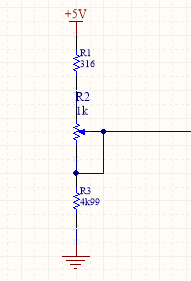
\includegraphics[scale=0.8]{Etapa-de-entrada.png}
	\caption{ Etapa de entrada.}
	\label{fig:etapa-de-entrada}
\end{figure}

 
 \noindent Se utiliza una resistencia variable de $1\:k\Omega$ y dos con valores fijos. Para poder excursionar la tensión de referencia entre $3.92\:V$ y $4.7\:V$, los valores de las resistencias $R_1$ y $R_3$ deben ser de $4911\:\Omega$ y $313.5\:\Omega$ respectivamente. 
 
\noindent Por lo tanto, al adoptar un valor comercial para ellas, resulta en $R_1 = 316 \:\Omega$ y en $R_3 = 4990 \:\Omega$.
 
\noindent De esta forma, el valor de tensión máximo para la referencia de posición queda en $4.69\:V$ y el mínimo en $3.96\:V$.
 
